\chapter*{Zeitmanagement}
	\documentPartEntry{Zeitmanagement}
	%TODO: Kapitel und Bild unten mit den letzten Erkenntnissen und erfassten Zeiten nochmals überarbeiten!
	Zur zeitlichen Planung und für die Auswertung der Arbeitszeit haben wir das \ppt\ Jira\footnote{\url{https://de.atlassian.com/software/jira}} verwendet,
	wie wir es auch für das ganze Projektmanagement verwendet haben.
	Wann immer wir einen Task erstellten, haben wir auch die dafür benötigte Dauer geschätzt
	und diese im Jira eingetragen.
	Gleichzeitig haben wir auch die effektive benötigte Zeit gebucht.
	Ein Beispiel für eine Erfassung von Arbeitszeit ist in Abbildung\ \ref{fig:logWork} abgebildet.
	
	\begin{figure}[H]
		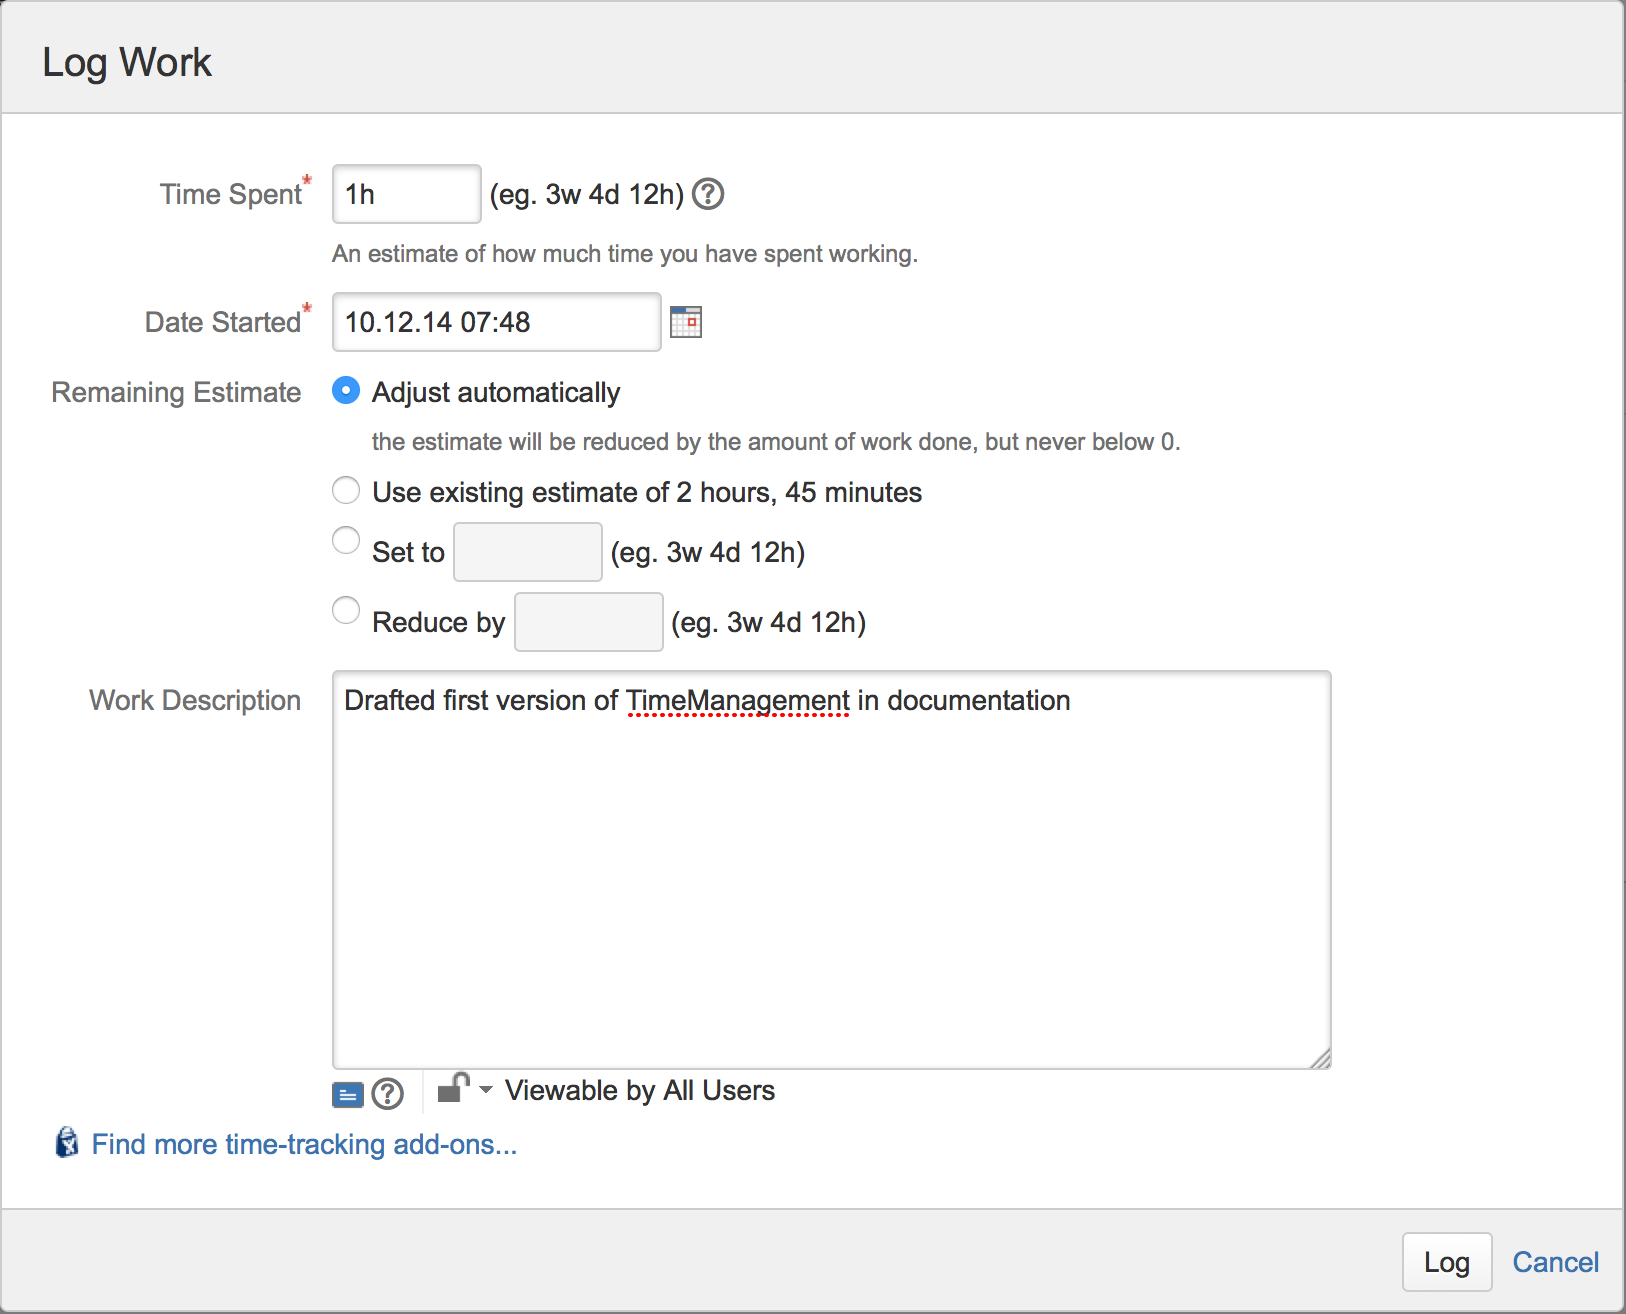
\includegraphics[width=0.5\textwidth]{projectPlan/media/img/logWork.png}
		\centering
		\caption{Erfassen von Arbeitszeit im Jira}
		\label{fig:logWork}
	\end{figure}
	
	Die erfassten Arbeitszeiten haben wir mit einem eigenen Ruby-Skript über die REST API von Jira\footnote{\url{https://docs.atlassian.com/jira/REST/latest/}} exportiert
	und in einer Excel-Tabelle jeweils laufend während dem Projekt ausgewertet.
	Grund dafür ist die dafür Fehlende Funktion im Basispaket von Jira\footnote{Es gibt eine kostenpflichtige Erweiterung, die Reporting anbietet}.
	Entstanden ist folgener Graph über die geleistete Arbeit in Abbildung\ \ref{fig:workGraph}.
	Darin sieht man den kontinuierlichen Verlauf während dem Projekt
	und die ausgeglichene Arbeitslast zwischen Tobias Blaser und Laurin Murer.
	Bereits von Anfang der Projektplanung an war geplant, die Arbeit eine Woche fertig zu stellen, um einen Puffer zum Abgabetermin zu besitzen.
	
	Aus diesem Grund endet die Linie des Soll-Max auch zu dieser Zeit.
	Die beiden Soll-Linien geben die von der HSR vorgegebene minimal und maximal erwarteten Aufwände an.
	
	\begin{figure}[H]
		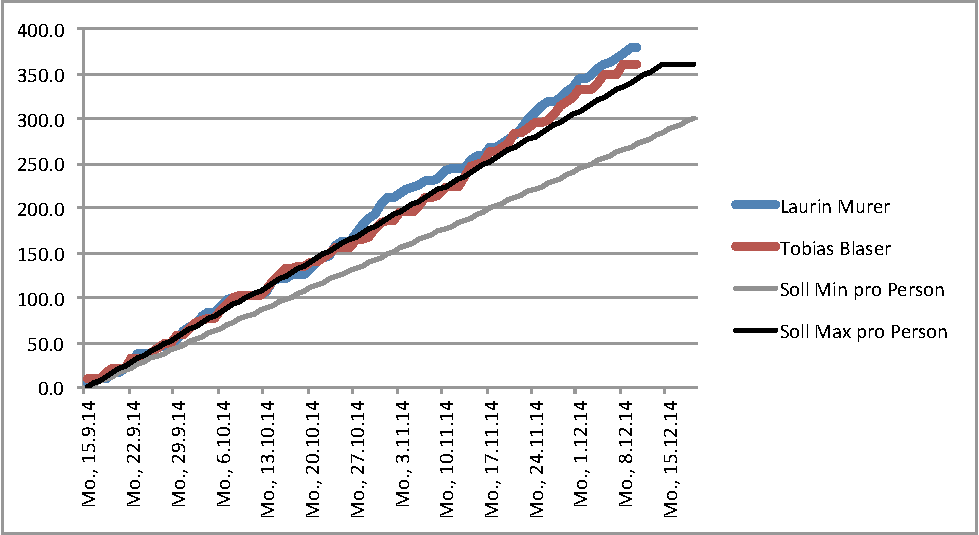
\includegraphics[width=\textwidth]{projectPlan/media/img/workGraph.pdf}
		\centering
		\caption{Graph über die geleistete Arbeit}
		\label{fig:workGraph}
	\end{figure}
	
	Wir haben von Begin des Projektes geplant, viel in das Projekt zu investieren, um ein Top-Ergebnis zu erreichen.
	
	Die gleichmässig steigenden Geraden zeigen auch,
	das sich unsere Projektplanung bewährt hat.


	\subsection{Schätzgenauigkeit der Aufwände}
	Wenig verwunderlich liegt die Schätzgenauigkeit bei kleinen Paketen nahe bei der effektiv benötigten Zeit.
	Bei grösseren Paketen ist die Differenz grösser und schwankt zwischen 50\% weniger und 100\% mehr benötigte Zeit als Extremwerte.
	Wir haben dabei häufiger den Aufwand überschätzt als unterschätzt.
	Nach Hochrechnungen liegt die durchschnittlich geschätzte Dauer zwischen 80\% und 100\% der effektiv benötigten Zeit.
	
	In dieser Rechnung nicht miteingeschlossen sind neu erstellte Issues aufgrund der Notwendigkeit der Umsetzung weiterer Teilaspekte eines grösseren Issueblockes.
	Würde man dies mitberücksichtigen, so liegt die effektiv benötgte Zeit schätzungsweise zwischen 20\% und 40\% über der geschätzten Zeit.
	Aufgrund dieser Erkenntnis in den ersten Wochen haben wir für die restlichen Milestones jeweils maximal 2/3 der Zeit für Features eingeplant und die Restliche Zeit einerseits für Administrative Tätigkeiten andererseits als Puffer vorgesehen, was sich bewährt hat. 
